%!TEX root = ../../thesis.tex

\section{Post reduction stages}
\label{sec:posreduction}
From the {DRACS} pipeline the 1-D spectra of each target has been extracted.
However, the spectra still need to undergo some post-extraction steps.
In particular, wavelength calibration and telluric correction.
A detailed look of how these steps were developed and performed are addressed in the following section.

\subsection{Wavelength calibration}
\label{subsec:wavecalib}
Wavelength calibration is the process of assigning accurate wavelength values to each pixel in the spectra.
For {CRIRES} in the \nir{} this is challenging.
{CRIRES} uses a Thorium-Argon (\thar) lamp to place 6 emission spectra on the detector using fibres.
The spectra of the \thar{} emission lines are used to determine the spatial distribution of the wavelength solution across each detector using correlation with a spectral template.
\thar{} lamps are excellent at optical wavelengths where the numerous (several thousand) spectral lines enable radial velocity precisions of sub\,-\mps{} when combined together, e.g. in the {HARPS} spectrograph.
The precision of an individual \thar{} line is of the order of \mps{}.

However, in the \nir{} there is a relatively low density of \thar{} lines~\citep{kerber_laboratory_2009}, which, in combination with the alignment of the narrow wavelength range of the detector, causes a poor wavelength calibration to be obtained (e.g.\ {CRIRES}-POP~\citep{nicholls_crirespop_2017}).
Above 2.2\um{} there are {O-H} sky lines that can be used for wavelength calibration but according to the {CRIRES} manual for observations below 2.2\um{} they are too dim.
These wavelength calibration issues were experienced when using the {ESO} {CRIRES} pipeline, with non-\thar{} features sometimes affecting the correlation.

Between the wavelength range 2.1--2.17\um{} there are roughly 80 \thar{} lines across all four detectors, as seen in \cref{fig:caliblamps}.
The {DRACS} pipeline does not use the \thar{} lamp files for wavelength calibration and leaves this as a post reduction step.

A common method for wavelength calibration that does not rely on \thar{} lamps of {CRIRES} involves using the telluric lines present to provide the wavelength solution~\citep[e.g.][]{brogi_signature_2012,brogi_carbon_2014,dekok_detection_2013,piskorz_evidence_2016}.
This is made possible by the use of high resolution spectra, in which the telluric lines are well resolved, as well as accurate spectral information of the atmosphere.

Likewise, in this work the wavelength calibration is performed using the telluric absorption lines present in each observation as the wavelength reference.
Instead of directly using the {HITRAN} database~\citep{rothman_hitran2012_2013} for the telluric line positions, such as~\citet[][]{brogi_signature_2012, brogi_carbon_2014, dekok_detection_2013}, use the {TAPAS} atmospheric transmission models (see \cref{sec:telluric_correction}).
The {TAPAS} models use the {HITRAN} database but also includes atmospheric profiles and physical meteorological measurements to model the telluric absorption strength.

To calibrate the wavelength the telluric lines in the model need to be associated to the corresponding telluric lines in the observed spectrum.
The centroid\footnote{Centre of the line} of each telluric line in the model is obtained by fitting the telluric transmission spectrum, \(T(\lambda)\), as a simple sum of Gaussian functions (subtracted from the continuum):
\begin{equation}
T(\lambda) = 1 - {\Sigma}_{i}\ G(\lambda, A_{i}, {\mu}_{i}, {\sigma}_{i}),
\end{equation}
where \(G\) is a Gaussian function of the form
\begin{equation}
G(\lambda, A, \mu, \sigma) = {A \textrm{e}}^{{-(\lambda-\mu)}^{2}/2\sigma^{2}},
\end{equation}
and \(A\), \(\mu\), \(\sigma\) are the amplitude, central wavelength, and standard deviation for each line respectively.
Telluric lines actually have a Voigt profile\footnote{A Voigt profile is a convolution of two broadening profiles, a Gaussian and a Lorentzian.
Gaussian broadening results from thermal Doppler broadening, and instrumental broadening while the Lorentzian broadening comes from molecular vibrational bands\citep{meier_art_2005}.} although they are not fully resolved in the \nir{} and their shape is dominated by the instrumental profile.
\citet{seifahrt_synthesising_2010} measured the instrumental profile of {CRIRES} using singular-value decomposition and showed that it is extremely well represented by a single Gaussian below a \snr{}$\sim$300.
Therefore, wavelength calibration using single Gaussian fits to each line is sufficient.

The observed spectra contain two different spectral components: stellar and telluric lines, which are multiplied together: The observed spectra are therefore fitted with a multiplication of two Gaussian-sum models.
\begin{align}
I_{obs}(x) &= {I}_{tell}(x) \times {I}_{star}(x) \nonumber\\
I_{obs}(x) &= {\Big(1 - {\Sigma}_{j}\ G(x, A_{j}, {\mu}_{j}, {\sigma}_{j})\Big)}_{tell} \times {\Big(1 - {\Sigma}_{k} G(x, A_{k}, {\mu}_{k}, {\sigma}_{k})\Big)}_{star}, \label{eqn:obs}
\end{align}
where \(x\) is the pixel coordinates of the extracted spectra.

The identification between telluric and stellar lines is performed by hand for each spectra, using the telluric model as the reference.
Care was taken to fit the correct components to blended spectra where possible to improve the number telluric lines use for calibration.
The fits were inspected to ensure that they reasonably matched the line positions.
There was difficulty in identifying the shallow lines with depths below 1--2\%, but these were needed in some spectra to obtain a suitable fit.
If there were blended lines that did not appear to fit correctly they were not considered in the calibration step.

After fitting \(I_{obs}(x)\) to the observed spectrum and \(T(\lambda)\) to the telluric model, the wavelength solution was obtained by fitting a second order polynomial to the centroid values \(\{\mu_{j}(x), \mu_{i}(\lambda)\}\) from the telluric components of the observed spectra and telluric model respectively.
A second order polynomial has been shown to be sufficient for higher precision {RV} studies~\citep[e.g.][]{bean_groundbased_2010, figueira_radial_2010}.
This polynomial is then used to map the whole spectrum from pixels into wavelength.
Higher \(3^{\textrm{rd}}\) and \(4^{\textrm{th}}\) order polynomials that are also used in the literature~\citep[e.g.][]{seifahrt_synthesising_2010, ulmer-moll_telluric_2018} were attempted but had limited success here due to the limited number and uneven spacing of telluric lines in the narrow wavelength range analysed, especially on the second detector.
There were often large deviations due to the uneven spread of telluric lines, especially at the extremities.
Higher order terms for wavelength calibration are usually used in regions with a higher density of telluric lines and/or a longer wavelength span~\citep{piskorz_evidence_2016, seifahrt_synthesising_2010, ulmer-moll_telluric_2018}.

\begin{figure}
    \centering
    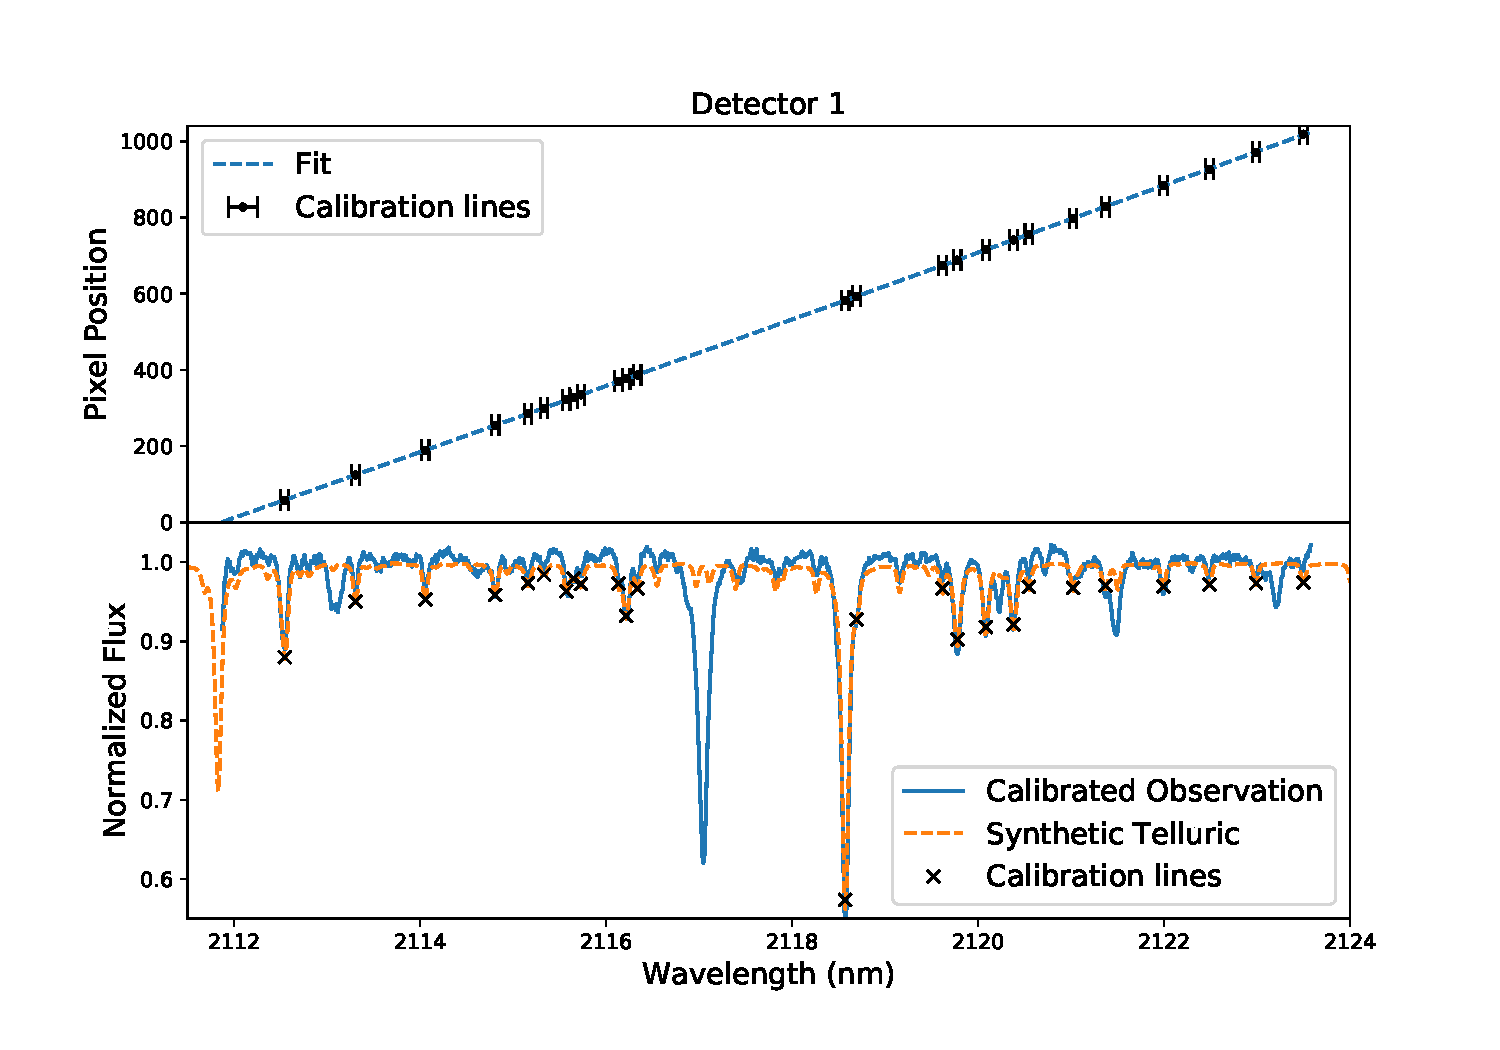
\includegraphics[width=0.85\linewidth]{figures/reduction/calibration.pdf}
    \caption[Example of the wavelength calibration using the synthetic telluric spectra.]{Example of the wavelength calibration using the synthetic telluric spectra.
        Top: The pixel/wavelength mapping and associated wavelength fit.
        The horizontal error bars shown are the Gaussian line width, around 0.04\nm{}.
        Bottom: The wavelength calibrated observation and the telluric model used for calibration.
        The black crosses indicate the peaks of the telluric lines used in the fitting process.}
    \label{fig:wl_calibration}
\end{figure}

An example of the wavelength fitting is given in \cref{fig:wl_calibration}.
The top panel shows the (slightly) quadratic fit (blue dashed) to the centroid values \(\{\mu_{j}(x), \mu_{i}(\lambda)\}\)(black) while the bottom panel shows the newly calibrated observation alongside the telluric spectrum.
The black crosses indicate the lines used for calibration.
To two decimal places the equation of the fit $\lambda = -1.85e^{-7} x^2 + 1.16e^{-2} x + 2111.86$.

Much like with the \thar{} calibrations, this technique performs better when there is sufficient coverage of telluric lines on the detectors.
For the wavelength setting of these observations, the spectra from the second detector (top right panel of \cref{fig:spectraexamples}) only has two large telluric lines present with several small lines, with relative depths smaller than 1\%, which are often difficult to accurately identify.
This deteriorated the calibration stability for the second detector.
The second detector may have been ideal for the detection of a faint secondary spectra, with the lack of telluric contamination and stellar lines.
Unfortunately the wavelength calibration quality varies in an inverse way, being more difficult with few lines.

It is noted that there are many variations on this wavelength calibration technique including those integrated within programs such as \emph{TelFit}~\citet{gullikson_correcting_2014}, and {ESO}'s \emph{Molecfit}~\citet{smette_molecfit_2015}, that perform telluric correction and re-calibrate the wavelength axis themselves at the same time.
It is recommended to attempt using those first before independently creating wavelength calibration software.

One improvement could have been to include a concurrent fitting of a stellar spectral model, adjusted for {RV}, along with the telluric model, which could help to improve the wavelength calibration performed here.
\citet{piskorz_evidence_2016} performed wavelength calibration using only a telluric line model at other \nir{} wavelengths (\emph{L}-band between 3.0--3.4\um{}) successfully.
However, around 2\um{} they needed to include a fitted stellar model to obtain good wavelength calibration due to the weaker telluric lines in this region.
This is the same wavelength region of the data analysed here.
Having experience of performing wavelength calibration at other wavelengths may have revealed the difficulties of calibration from the telluric lines at 2\um{} sooner.

A brief attempt of wavelength calibration using the iterative calibration method outlined in~\citet{brogi_rotation_2016} was made.
This involved generating a set of quadratic wavelength solutions for the observed spectrum and cross-correlating each one against the telluric model.
The solutions for the next iteration are obtained by refining the parameters from the wavelength solution with the highest correlation.
The method worked well for~\citet{brogi_rotation_2016} as they included templates for both the star and telluric lines and they were observing in a wavelength domain in which there is a large number of strong and uniform stellar \ce{CO} lines across the detector.
The brief experiments with this method were not successful as they did not include a stellar model or mask, which lead to incorrect fitting solutions.
Without adding any stellar masking the telluric lines would strongly correlate to the stellar lines present, especially where there were blended lines.
This lead to visibly incorrect wavelength solutions and this method was abandoned.
If a stellar mask was used it may have been possible to achieve more sensible results, although still challenging to the low density of telluric lines at this wavelength range.

At one point it was considered to attempt a global fit of the wavelength calibration, using all four {CRIRES} detectors together.
This would create a consistent fit to the dispersion across all 4 detectors at once.
This would require extra fitting parameters to define the size of the 3 gaps between the detectors and any vertical offsets.
This fit may even need to be performed on the two-dimensional images, before the 1-D extraction.
This may have allowed for the telluric lines from neighbouring detectors to help fit the calibration on detectors where there are very few telluric lines (e.g.\ detector \#2).
The fitted instrument parameters such as the detector gaps may even be constrained so that they are physically consistent across all observations.
However, this idea was not explored further or implemented due to time constraints.
An example of the wavelength calibration using all four detectors is provided in \cref{appendix:wavelength_fitting}.
In the future it may be possible or necessary to combine all of the methods above, including the \thar{} calibration lines, telluric models, stellar templates, and multiple detectors fitted at once to achieve precise wavelength calibration.

\begin{figure}
    \centering
    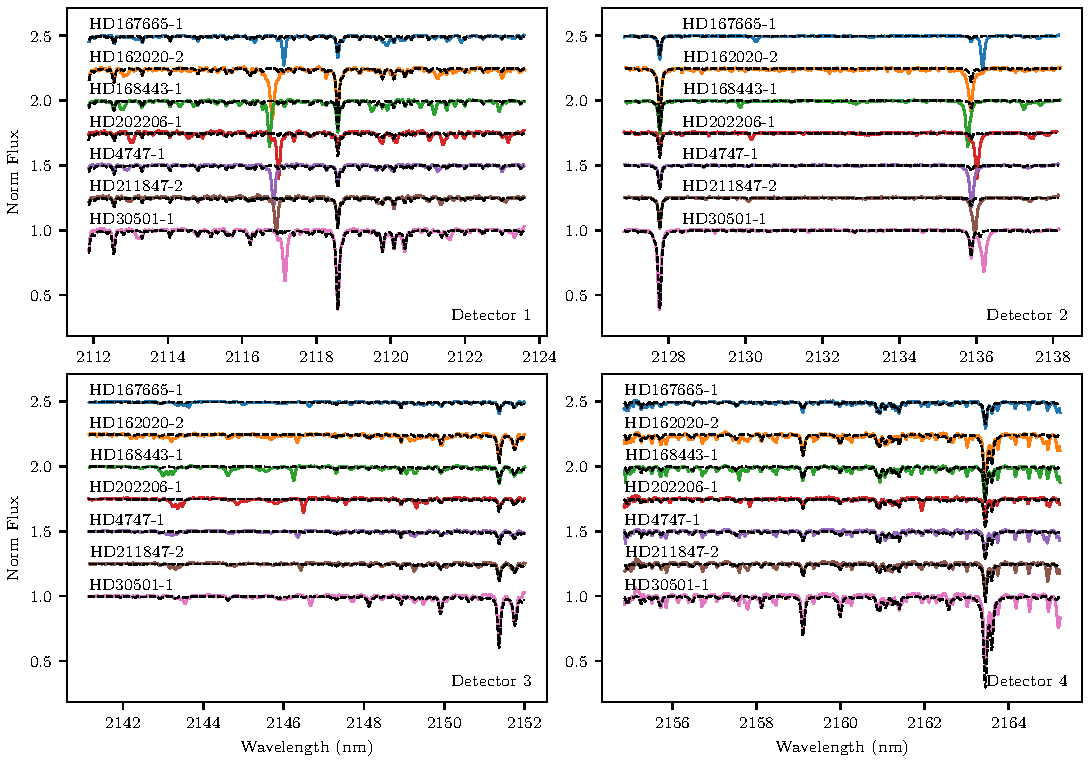
\includegraphics[width=1\linewidth]{figures/reduction/Spectra_examples}
    \caption[Example reduced CRIRES spectra for each target.]{An example spectra for each target and each detector \#1--4 in order of increasing wavelength.
       The solid lines are the spectra while the black dashed lines are the telluric models used for wavelength correction, showing good alignment with the spectra.}
    \label{fig:spectraexamples}
\end{figure}

In hindsight using the wavelength solution from the {ESO} pipeline, or the linear solution from the CRIRES manual, may have been good starting points, rather than the pixel positions, for calibration of the {DRACS} reduced spectra.
This may have made the line identification simpler.

In simulations of a differential technique similar to what is presented in \cref{cha:direct_recovery}, \citet{kostogryz_spectral_2013} simulate the affect of wavelength calibration errors on differential result.
They found that calibration error >0.1 pixels will produce signals greater than the photon noise level in spectra with a \snr{} of around 500.
They show that this upper limit only just the level achieved by~\citep{brogi_signature_2012} calibrated using the telluric lines from the observation.
This shows how important the wavelength calibration is to detect the spectra of the companion.


\subsection{Telluric correction}
\label{subsec:telluric_correction_application}
Correction of the telluric lines is performed after wavelength correction, using the same {TAPAS} models.
When inspecting the models and observations there was slight difference in the airmass, $m$, between the synthetic spectra and the airmass in the fits header.
The depth of the telluric lines were re-scaled to match the airmass of the observations using the relation \(\rm T = T^{\beta}\), where \(\rm T\) is the transmission of the telluric spectrum and \(\beta\) is the airmass ratio between the observation and model $\beta ={m_{observed}/m_{model}}$.
This scaling adjusted the depth of most absorption lines to better match the observations, but does not correctly scale the deeper \ce{H2O} lines, for which there were still differences.

The scaled telluric model is interpolated to the wavelengths of the observed spectrum and then used to correct the observed spectra through division, leaving behind a telluric corrected spectra.
Telluric spectra used for correction can be observed alongside the non-corrected spectra in \cref{fig:spectraexamples} as the black dashed lines.

\subsubsection{Separate \ce{H2O} scaling.}
A technique suggested by~\citet{bertaux_tapas_2014} was attempted to address the poor \ce{H2O} airmass scaling.
This involved fitting a scaling factor to the \ce{H2O} absorption lines before convolution to the instrument resolution.
This was achieved by first dividing the spectrum by a telluric model containing the non-\ce{H2O} constituents, convolved to the observed resolution, and scaled by the airmass to remove the non-\ce{H2O} lines.
Then the telluric model with only \ce{H2O} lines at full resolution was scaled by a factor \(\textrm{T}^{x}\) and convolved to the instrumental resolution\footnote{\(\rm R=50\,000\) for this work} and compared to the remaining telluric lines in the observed spectra.
This scaled and convolved model was fitted to the observations to find the best was fitted to find the best scaling factor \(x\), for the \ce{H2O} lines.

It was found that for a few spectra in the sample this method corrected the deeper telluric lines well, but in many cases the fitted scaling factor was affected by the presence of blended stellar lines (attempting to fit those also).
It was also strongly influenced by the deepest \ce{H2O} telluric lines present.
The telluric correction of the deep \ce{H2O} lines could be improved with this technique, but at the cost of worsening the correction of the many smaller \ce{H2O} lines.
Since the smaller \ce{H2O} lines covered more of the spectrum in this region than the larger lines, the separate \ce{H2O} scaling was not continued.
One possible solution for this would be to perform a piece-wise telluric correction, performing this step only for the deeper \ce{H2O} lines.
This technique could also benefit from a larger wavelength span that would enable blended lines to be ignored while having sufficient deep \ce{H2O} lines to fit the scaling factor correctly.
This small experiment shows that a simple scaling is not enough to correct for the absorption of \ce{H2O} in an effective way, for this case.
Another better solution would be using proper atmospheric fitting tools that fits the telluric model to the observations, such as {Molecfit}, in which the atmospheric composition can be changed to match the observed telluric line strengths.


\subsection{Wavelength masking}
Throughout the course of this work several wavelength regions were found where the extraction could not be performed reliably due to the wavelength calibration and telluric line corrections.
Different wavelength masks are applied to these areas to remove them from the spectra.
The main reasons that wavelength masking is used are collated below.

Firstly, regions near the edges of each detector where the wavelength solution is extrapolated outside of the calibrating telluric lines are removed, reducing the effective size of each detector by about \(10\%\) or \(\sim\)100 pixels.

Secondly, any remaining artefacts present in the spectra and the centres of deep telluric lines where telluric correction was not corrected properly are masked out.
The telluric correction sometimes results in ``emission-like'' peaks in the corrected spectrum, which are removed.
These factors combined result in masking out around a further 10\% of the observed spectra.

In \cref{sec:chi2_results} a further wavelength restriction is applied to mask out regions where there is a large mismatch between the observed spectrum and the closest synthetic spectra to the host.
This significantly restricts the wavelength span utilized for that purpose to around only 43\%.
The masked regions created by this last mask are shown in \cref{fig:visualinspection-hd2118471}.


\subsection{Barycentric {RV} correction}
\label{subsec:barycentriccorrection}
After the telluric correction is performed, the spectra are corrected for Earth's barycentric motion.
The orbital and rotational motion of the Earth imparts a daily and seasonal radial velocity measurement offset onto observations.
To accurately compare the radial velocity (or spectral shift) between two measurements, they need to be translated into a common rest frame.
The rest frame of choice is the barycentre of the Solar System.
Equations to relate the observed spectral shift to the {RV} shift at the \textit{Barycentric Celestial Reference Reference System}~\citep{rickman_transactions_2001} rest frame are provided in~\citet{lindegren_fundamental_2003}.

In this work the barycentric velocity correction is calculated using PyAstronomy's\footnote{https://pyastronomy.readthedocs.io} \emph{helcor} function ported from the REDUCE IDL package (see~\citet[][]{piskunov_new_2002}).
This calculates radial velocity of the observer towards the astronomical target, accounting for Earth's barycentric motion as well as Earth's rotation, to the accuracy of \(\sim\)1\mps{}.
This computation requires the date and time of the observation, the location of the observatory and the celestial coordinates of the target.
The observed spectra are Doppler shifted by the negative value of the barycentric velocity calculated, placing all spectra as if they were observed from the barycentre of the Solar System.

The maximum barycentric velocity of the Earth is around 30\kmps{}.
Spectral regions within $\pm30$\kmps{} of telluric lines with an absorption depth >2\% are commonly masked out to avoid them in analyses (such as {RV} determination), as these regions will overlap and be affected by the telluric lines at some point during the year.
